\section{Metodi di iterazione funzionale}
Per trovare altri metodi, differenti da quello di bisezione, possiamo osservare che la nostra funzione
$f(x) = 0$ possiamo riscriverla in diversi modi:
\begin{align*}
	x = & x - f(x)              \\
	x = & x - \frac{f(x)}{h(x)}
\end{align*}
dove $h$ è una funzione definita sugli \emph{zeri} di $f$. Questo ci dice che il problema di trovare $x$ tale
che $f(x) = 0$ lo possiamo vedere come il problema nel trovare $x$ tale che
\[ x = g(x) \]
dove $g(x)$ potrebbe essere $x - f(x)$ oppure $x - \frac{f(x)}{h(x)}$. Posto in questi termini il problema non
è più quello di trovare gli zeri di $f$ ma diventa quello di trovare i \textbf{punti fissi} di $g$, ossia quei
punti $x$ di $g$ che si mandano in se stessi.

Questa equivalenza è interessante poiché ci permette di vedere il problema in questo modo
\[
	\begin{cases}
		x_0 \in [a, b] \\
		x_{k+1} = g(x_k)
	\end{cases}
\]
e possiamo dimostrare facilmente che se $g : \R \to \R$ è continua e
\[ \lim_{k \to +\infty} x_{k} = \alpha \]
allora $g(\alpha) = \alpha$, quindi $\alpha$ è un punto fisso di $g$ e uno zero di $f$.

\begin{example}
	Consideriamo l'equazione
	\[ \sqrt{x} - x = 0 \]
	Prima di tutto notiamo che la funzione è definita per $x \geq 0$ e poi, sviluppando l'equazione, possiamo
	scrivere
	\begin{align*}
		\sqrt{x} - x = & 0   \\
		\sqrt{x} =     & x   \\
		x =            & x^2 \\
		x^2 - x =      & 0   \\
		x (x - 1) =    & 0
	\end{align*}
	Ottenendo così le soluzioni $x = 0$ e $x = 1$. Notiamo però che l'equazione può essere scritta come
	\[ x = \sqrt{x} \]
	e quindi possiamo dire che
	\[ g_1(x) = \sqrt{x} \]
	Riconducendoci al sistema di prima possiamo scrivere
	\[ x_{k+1} = g_1(x_k) = \sqrt{x_k} \]
	prendendo un qualsiasi $x_0 \in \R^+$. Proviamo a capire a cosa converge la successione che calcoliamo.
	Prima di tutto disegnamo un grafico per la funzione $g_1$ e per la retta $x$
	\begin{center}
		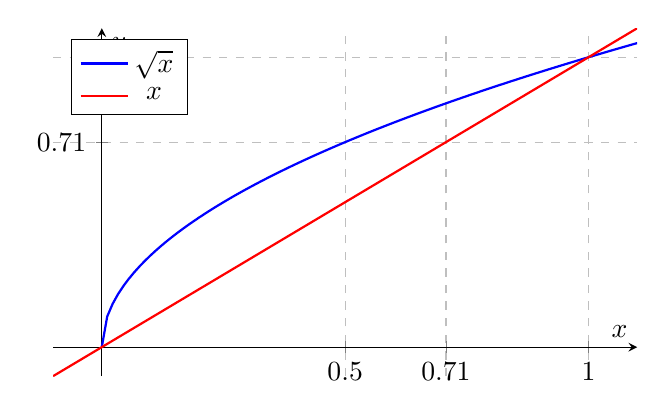
\begin{tikzpicture}
			\begin{axis}[
					font=\normalsize,
					width=9cm,
					height=6cm,
					axis lines = center,
					xlabel = $x$,
					ylabel = $y$,
					xtick = {1/2, sqrt(1/2), 1},
					ytick = {sqrt(1/2), 1},
					ymin = 0, ymax = 1,
					xmin = 0, xmax = 1,
					grid = both,
					grid style = dashed,
					legend pos = north west,
					enlargelimits
				]

				\addplot [
					domain=0:1.1,
					samples=100,
					thick,
					color=blue
				]
				{sqrt(x)};

				\addplot [
					domain=-0.1:1.1,
					samples=20,
					thick,
					color=red
				]
				{x};

				\legend{
					$\sqrt{x}$,
					$x$
				}
			\end{axis}
		\end{tikzpicture}
	\end{center}
	Scegliamo un $x_0$ compreso tra 0 e 1, supponiamo $\frac{1}{2}$, e proviamo a calcolare qualche $x_i$ per
	vedere come procede la successione. Come sappiamo, per calcolare $x_1$, dobbiamo applicare a $x_0$ la nostra
	funzione $g_1$. Otteniamo quindi
	\begin{gather*}
		x_1 = \sqrt{x_0} = \sqrt{0.5} = 0.71 \\
		x_2 = \sqrt{x_1} = \sqrt{0.71} = 0.84
	\end{gather*}

	\begin{center}
		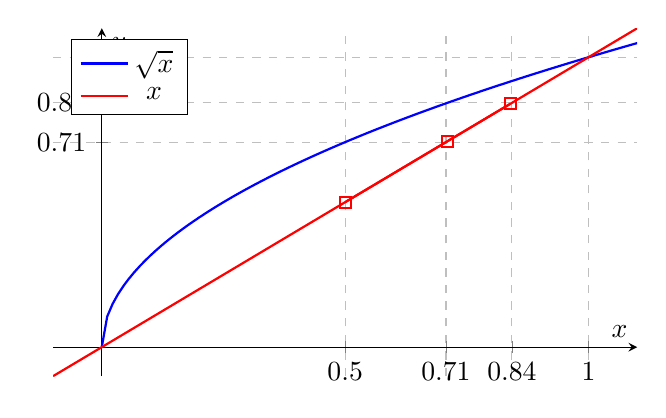
\begin{tikzpicture}
			\begin{axis}[
					font=\normalsize,
					width=9cm,
					height=6cm,
					axis lines = center,
					xlabel = $x$,
					ylabel = $y$,
					xtick = {1/2, sqrt(1/2), sqrt(0.71), 1},
					ytick = {sqrt(1/2), sqrt(0.71), 1},
					ymin = 0, ymax = 1,
					xmin = 0, xmax = 1,
					grid = both,
					grid style = dashed,
					legend pos = north west,
					enlargelimits
				]

				\addplot [
					domain=0:1.1,
					samples=100,
					thick,
					color=blue
				]
				{sqrt(x)};

				\addplot [
					domain=-0.1:1.1,
					samples=20,
					thick,
					color=red
				]
				{x};

				\addplot [
					domain=-0.1:1.1,
					samples=20,
					thick,
					color=red,
					mark=square
				]
				coordinates { (1/2, 1/2) (0.71, 0.71) (0.84, 0.84) };

				\legend{
					$\sqrt{x}$,
					$x$
				}
			\end{axis}
		\end{tikzpicture}
	\end{center}
	Andando avanti ci si accorge che se $0 < x_0 < 1$ allora $x_k$ tende a 1 per $k \to +\infty$. Se definiamo
	$x_0 > 1$ la situazione non cambia. Supponiamo di scegliere $x_0 = 1.1$, la successione che calcoliamo è
	la seguente
	\begin{gather*}
		x_1 = \sqrt{1.1} = 1.05  \\
		x_2 = \sqrt{1.05} = 1.02
	\end{gather*}
	Graficamente otteniamo questo tipo di successione
	\begin{center}
		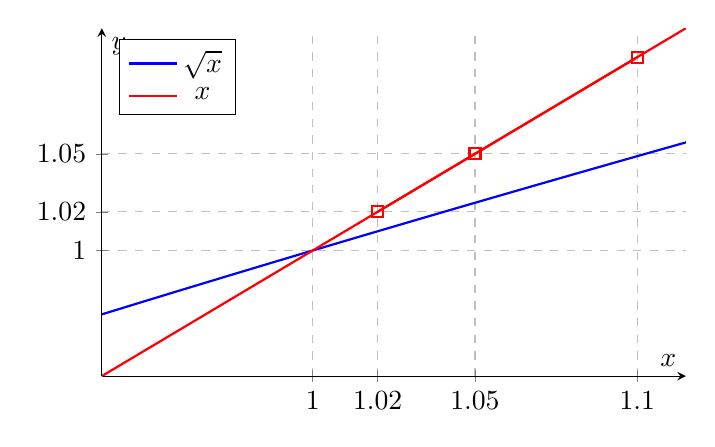
\begin{tikzpicture}
			\begin{axis}[
					font=\normalsize,
					width=9cm,
					height=6cm,
					axis lines = center,
					xlabel = $x$,
					ylabel = $y$,
					xtick = {1, 1.1, 1.05, 1.02},
					ytick = {1, 1.05, 1.02},
					ymin = 0.95, ymax = 1.1,
					xmin = 0.95, xmax = 1.1,
					grid = both,
					grid style = dashed,
					legend pos = north west,
					enlargelimits
				]

				\addplot [
					domain=0:1.2,
					samples=100,
					thick,
					color=blue
				]
				{sqrt(x)};

				\addplot [
					domain=0:1.2,
					samples=20,
					thick,
					color=red
				]
				{x};

				\addplot [
					domain=0.9:1.3,
					samples=20,
					thick,
					color=red,
					mark=square
				]
				coordinates { (1.1, 1.1) (1.05, 1.05) (1.02, 1.02) };

				\legend{
					$\sqrt{x}$,
					$x$
				}
			\end{axis}
		\end{tikzpicture}
	\end{center}
	Come possiamo vedere, anche in questo caso la successione converge a 1 per $k \to +\infty$. In generale
	possiamo osservare che, a meno che non scegliamo $x_0 = 0$, il metodo converge sempre a 1 anche se scegliamo
	$x_0$ molto vicino a 0. Se consideriamo un'equazione equivalente a $x = g_1(x)$, supponiamo $g_2(x) = x^2$
	e quindi
	\[ x = g_2(x) = x^2 \]
	calcoleremo la successione in questo modo
	\[ x_{k+1} = x_k^2 \]
	In questo caso, possiamo osservare come il metodo converga a 0 per $x_0 < 1$. Al contrario per $x_0 > 1$ il
	metodo diverge. Supponiamo ad esempio $x_0 = 0.5$ e facciamo due iterazioni
	\begin{gather*}
		x_1 = 0.5^2 = 0.25 \\
		x_2 = 0.25^2 = 0.625
	\end{gather*}
	Se invece scegliamo ad esempio $x_0 = 1.1$, dopo due iterazioni otteniamo
	\begin{gather*}
		x_1 = 1.1^2 = 1.21 \\
		x_2 = 1.21^2 = 1.46
	\end{gather*}
\end{example}

Questo esempio ci fa capire che abbiamo bisogno di un criterio per determinare delle condizioni di convergenza
indipendenti dalla scelta del punto iniziale.

\subsection{Convergenza}
Cerchiamo quindi di individuare dei criteri in grado di stabilire delle condizioni di convergenza per i metodi
che scegliamo di implementare.

\begin{theorem}[Punto fisso]\label{th: punto_fisso}
	Sia $g : [a, b] \to \R$ di classe $C^1 ([a, b])$ e sia $g(\alpha) = \alpha$ con $\alpha \in (a,b)$. Se esiste
	$\rho > 0$ tale che $|g'(x)| < 1$ per ogni $x \in [\alpha - \rho, \alpha + \rho] = I_\alpha$ allora la
	successione generata dal metodo
	\[ x_{k+1} = g(x_k) \]
	a partire da $x_0 \in I_\alpha$ soddisfa queste due proprietà
	\[ x_k \in I_\alpha \quad \wedge \quad \lim_{k \to +\infty} x_k = \alpha \]
	\begin{proof}
		La dimostrazione procede per induzione. Iniziamo col dire che noi sappiamo per ipotesi che esiste un
		intorno circolare dove $|g'(x)| < 1$. Dato che la derivata prima è una funzione continua, il modulo
		della derivata prima è ancora continua.

		Per il teorema di Weierstrass sappiamo che una funzione continua in un intervallo chiuso e limitato
		ammette massimo e minimo. Esiste quindi il massimo $\lambda$ di $|g'(x)|$ per $x \in I_\alpha$.
		Dato che $|g'(x)| < 1$ anche $\lambda < 1$.

		A questo punto noi vogliamo dimostrare per induzione che gli elementi della successione soddisfano
		questa proprietà:
		\[ |x_k - \alpha| \leq \lambda^k \rho \quad \forall k \geq 0 \]
		Dato che $\lambda < 1$ vale che
		\[ |x_k - \alpha| \leq \lambda^k \rho \leq \rho \quad \Rightarrow \quad x_k \in I_\alpha \]
		Consideriamo anche
		\[ 0 \leq |x_k - \alpha| \leq \lambda^k \rho \]
		Dato che
		\[ \lim_{k \to +\infty} \lambda^k \rho = 0\]
		allora, per il teorema dei carabinieri, anche
		\[ \lim_{k \to +\infty} |x_k - \alpha| = 0 \]
		e quindi $x_k \to \alpha$. Per riuscire a dimostrare la proprietà per induzione procediamo in questo modo:
		\begin{enumerate}
			\item Il passo base consiste nel dimostrare che
			      \[ |x_0 - \alpha| \leq \lambda^0 \rho = \rho \]
			      ma questo è vero per ipotesi poiché $x_0 \in I_\alpha$.
			\item Supponiamo ora di aver dimostrato fino all'ordine $k$ e cerchiamo di dimostrare che
			      \[ |x_{k+1} - \alpha| \leq \lambda^{k+1} \leq \rho \]
			      Dato che $x_{k+1} = g(x_k)$ e $\alpha$ è un punto fisso di $g$ possiamo scrivere
			      \[ |x_{k+1} - \alpha| = |g(x_k) - g(\alpha)| \]
			      A questo punto possiamo applicare il teorema di Lagrange, il quale ci dice che esiste un punto
			      $\xi_k$ tale che
			      \[ |g(x_k) - g(\alpha)| = |g'(\xi_k) (x_k - \alpha)| = |g'(\xi_k)| \cdot |x_k - \alpha| \]
			      dato che $|g'(\xi_k)| \leq \lambda$ e per ipotesi vale $|x_k - \alpha| \leq \lambda^k \rho$
			      allora vale
			      \[ |g'(\xi_k)| \cdot |x_k - \alpha| \leq \lambda \cdot \lambda^k \rho = \lambda^{k+1} \rho \]
		\end{enumerate}
	\end{proof}
\end{theorem}

Dato che la condizione $|g'(x)| < 1$ è \emph{difficile} da studiare su un intervallo, si da anche una versione
più debole del teorema il quale si occupa di verificare la proprietà nel punto $\alpha$.

\begin{corollary}\label{coro: punto_fisso}
	Sia $g : [a, b] \to \R$ di classe $C^1 ([a, b])$ e sia $g(\alpha) = \alpha$ con $\alpha \in [a,b]$. Se
	$|g'(\alpha)| < 1$ allora esiste un intervallo $I_\alpha = [\alpha - \rho, \alpha + \rho]$ tale che per
	ogni $x_0 \in I_\alpha$ valgono le seguenti proprietà:
	\begin{itemize}
		\item $x_k \in I_\alpha$ per ogni $k$.
		\item $x_k \to \alpha$.
	\end{itemize}
	\begin{proof}
		Prendiamo $h(x) = |g'(x)| - 1$ che è una funzione continua. Dato che $h(\alpha) = |g'(\alpha)| - 1$ e
		per le ipotesi del teorema vale che
		\[ |g'(\alpha)| - 1 < 0 \]
		Per il teorema di permanenza del segno esiste un intervallo $I_\alpha$ tale che
		\[ h(x) < 0 \quad \forall x \in I_\alpha \]
		il quale ci dice che se una funzione continua è negativa in un punto possiamo trovare circolare del punto
		in cui la funzione è negativa. Nel nostro caso dire che la funzione è negativa equivale a dire
		\[ h(x) < 0 \quad \Leftrightarrow \quad |g'(x)| < 1 \]
		Ecco le ipotesi del teorema \ref{th: punto_fisso} sono soddisfatte.
	\end{proof}
\end{corollary}

Il corollario \ref{coro: punto_fisso} ci dice che se $|g'(\alpha)| < 1$ allora il metodo è
\textbf{localmente convergente} in $\alpha$. Possiamo quindi trovare un intorno sufficientemente piccolo che
permetta la convergenza.

\begin{example}
	Vogliamo determinare quante soluzioni reali ha l'equazione
	\[ e^{-x} = x \]
	Procediamo per separazione grafica tracciando il grafico del sistema
	\[
		\begin{cases}
			y = e^{-x} \\
			y = x
		\end{cases}
	\]
	\begin{center}
		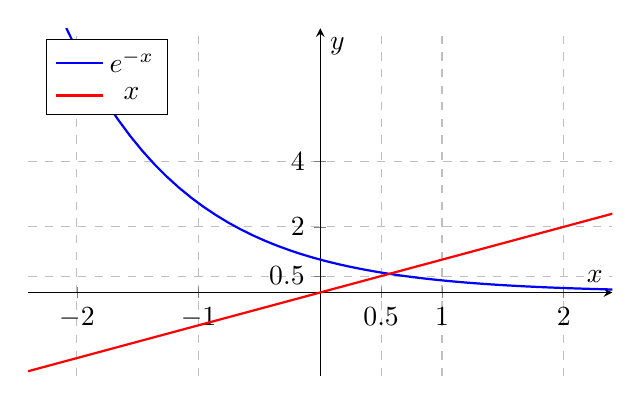
\begin{tikzpicture}
			\begin{axis}[
					font=\normalsize,
					width=9cm,
					height=6cm,
					axis lines = center,
					xlabel = $x$,
					ylabel = $y$,
					xtick = {-1, -2, 1, 0.5, 2},
					ytick = {0.5, 2, 4},
					xmin = -2, xmax = 2,
					grid = both,
					grid style = dashed,
					legend pos = north west,
					enlargelimits
				]

				\addplot [thick, color=blue, samples=100] {exp(-x)};
				\addplot [thick, color=red] {x};

				\legend{ $e^{-x}$, $x$ }
			\end{axis}
		\end{tikzpicture}
	\end{center}
	Possiamo quindi concludere che esiste ed è unica una soluzione $\alpha$ reale tale che
	\[ e^{-\alpha} = \alpha \]
	Tale soluzione è compresa tra 0 e un punto in cui la funzione $x$ vale di più della funzione $e^{-x}$.
	Se valutiamo le due funzioni per $x = 1$ otteniamo
	\[
		f(1) = \begin{cases}
			e^{-1} < 1 \\
			1
		\end{cases}
	\]
	Possiamo quindi concludere che $\alpha \in [0, 1]$. Per risolvere l'equazione non lineare consideriamo il
	metodo iterativo
	\[ x_{k+1} = g(x_k) = e^{-x_k} \]
	con $k \geq 0$ e vogliamo capire se il metodo è \emph{localmente convergente} in $\alpha$. Per riuscire a
	capirlo dobbiamo applicare il corollario \ref{coro: punto_fisso}.

	Per prima cosa verifichiamo che $g \in C^1([0, 1])$ ma questo è verificato poiché $e^{-x}$ è una funzione
	di classe $C^\infty(\R)$. Dobbiamo ora valutare $|g'(\alpha)|$
	\[ |g'(\alpha)| = |-e^{-\alpha}| = e^{-\alpha} \]
	ma dato che $\alpha$ è un punto fisso
	\[ e^{-\alpha} = \alpha \in (0, 1) \]
	Quindi anche senza conoscere $\alpha$ possiamo dire che
	\[ \alpha < 1 \quad \Rightarrow \quad |g'(\alpha)| < 1\]
	Ne concludiamo che il metodo è localmente convergente per $\alpha$.

	Se ora volessimo determinare un punto iniziale tale che il metodo sia convergente, ciò che abbiamo fatto
	fino ad ora non ci da alcuna informazione a riguardo. Dobbiamo quindi applicare il teorema
	\ref{th: punto_fisso}. Valutiamo quindi il modulo della derivata prima di $g(x) = e^{-x}$
	\[ |g'(x)| = |-e^{-x}| = e^{-x} \]
	e cerchiamo di capire per quali valori di $x$ vale
	\[ e^{-x} < 1 \]
	In questo caso possiamo facilmente dedurre che
	\[ e^{-x} < 1 \quad \Leftrightarrow \quad x > 0 \]
	Concludiamo quindi che possiamo prendere un qualsiasi intorno circolare di $\alpha$ contenuto nella semiretta
	positiva. Per trovare questo intorno procediamo valutando la funzione per esempio in $\frac{1}{2}$
	\[
		f \left( \frac{1}{2} \right) = \begin{cases}
			e^{-\frac{1}{2}} = \frac{1}{\sqrt{e}} \\
			\frac{1}{2}
		\end{cases}
	\]
	Dato che $\frac{1}{2} < \frac{1}{\sqrt{e}}$ significa che $\alpha$ è più vicino a 1 che a 0 e quindi possiamo
	prendere $\rho = 1 - \alpha$ e muoverci nell'intorno circolare centrato in $\alpha$
	\[ I_\alpha = [\alpha - \rho, \alpha + \rho] = [2\alpha - 1, 1] \]
\end{example}

\begin{definition}
	Il corollario \ref{coro: punto_fisso} ci permette di definire una casistica per i punti fissi:
	\begin{itemize}
		\item Se $|g'(\alpha)| < 1$ il punto fisso $\alpha$ è detto \textbf{attrattivo}.
		\item Se $|g'(\alpha)| > 1$ il punto fisso $\alpha$ è detto \textbf{repulsivo}.
		\item Se $|g'(\alpha)| = 1$ non possiamo dire niente, il punto potrebbe essere attrattivo o repulsivo. Per
		      determinarlo serve un'analisi più accurata.
	\end{itemize}
\end{definition}

\begin{example}
	Vogliamo capire se la radice $\alpha$ dell'equazione
	\[ e^{-x} = x \]
	è un punto attrattivo o repulsivo per il metodo
	\[ x_{k+1} = g(x_k) = -\ln (x_k) \]
	con $k \geq 0$. Prima di tutto calcoliamo la derivata della funzione $g$
	\[ g'(x_k) = -\frac{1}{x_k} \]
	Valutiamo ora il modulo della derivata valutata in $\alpha$
	\[ |g'(\alpha)| = \left| -\frac{1}{\alpha} \right| = \frac{1}{\alpha} \]
	Come abbiamo visto nell'esempio precedente $0 < \alpha < 1$ quindi
	\[ \frac{1}{\alpha} > 1 \quad \Rightarrow \quad |g'(\alpha)| > 1 \]
	possiamo quindi concludere che $\alpha$ è un punto repulsivo per il metodo scelto.
\end{example}
